%%%%%%%%%%%%%%%%%%%%%%%%%%%%%%%%%%%%%%%%%
% University/School Laboratory Report
% LaTeX Template
% Version 3.1 (25/3/14)
%
% This template has been downloaded from:
% http://www.LaTeXTemplates.com
%
% Original author:
% Linux and Unix Users Group at Virginia Tech Wiki 
% (https://vtluug.org/wiki/Example_LaTeX_chem_lab_report)
%
% License:
% CC BY-NC-SA 3.0 (http://creativecommons.org/licenses/by-nc-sa/3.0/)
%
%%%%%%%%%%%%%%%%%%%%%%%%%%%%%%%%%%%%%%%%%

%----------------------------------------------------------------------------------------
%	PACKAGES AND DOCUMENT CONFIGURATIONS
%----------------------------------------------------------------------------------------

\documentclass{article}

\usepackage[version=3]{mhchem} % Package for chemical equation typesetting
\usepackage{siunitx} % Provides the \SI{}{} and \si{} command for typesetting SI units
\usepackage{graphicx} % Required for the inclusion of images
\usepackage{natbib} % Required to change bibliography style to APA
\usepackage{amsmath} % Required for some math elements 
\usepackage[table,xcdraw]{xcolor}
\usepackage{listings}
\usepackage{hyperref}
\usepackage{xcolor}
\usepackage{color} %red, green, blue, yellow, cyan, magenta, black, white
\definecolor{mygreen}{RGB}{28,172,0} % color values Red, Green, Blue
\definecolor{mylilas}{RGB}{170,55,241}
\lstset{language=Matlab,%
    %basicstyle=\color{red},
    breaklines=true,%
    morekeywords={matlab2tikz},
     backgroundcolor=\color{black!5}, % set backgroundcolor
    keywordstyle=\color{blue},%
    morekeywords=[2]{1}, keywordstyle=[2]{\color{black}},
    identifierstyle=\color{black},%
    stringstyle=\color{mylilas},
    commentstyle=\color{mygreen},%
    showstringspaces=false,%without this there will be a symbol in the places where there is a space
    numbers=left,%
    numberstyle={\tiny \color{black}},% size of the numbers
    numbersep=9pt, % this defines how far the numbers are from the text
    emph=[1]{for,end,break},emphstyle=[1]\color{red}, %some words to emphasise
    %emph=[2]{word1,word2}, emphstyle=[2]{style},    
}

\usepackage[utf8]{inputenc} %Türkçe karakterler
\usepackage{floatrow}
\usepackage{geometry}
\usepackage{caption}
\usepackage{subcaption}
\geometry{margin=1in}

\renewcommand{\lstlistingname}{Code Snippet}

%\setlength\parindent{0pt} % Removes all indentation from paragraphs

% Table float box with bottom caption, box width adjusted to content
\newfloatcommand{capbtabbox}{table}[][\FBwidth]


%\usepackage{times} % Uncomment to use the Times New Roman font

%----------------------------------------------------------------------------------------
%	DOCUMENT INFORMATION
%----------------------------------------------------------------------------------------

\title{Assignment 3: \\ Face Detection With A Sliding Window\\ COMP 408} % Title

\author{Ahmet \textsc{Uysal}} % Author name

\date{\today} % Date for the report

\begin{document}

\maketitle % Insert the title, author and date

\begin{center}
\begin{tabular}{l r}
Instructor: & Y\"ucel  \textsc{Yemez} % Instructor/supervisor
\end{tabular}
\end{center}

% If you wish to include an abstract, uncomment the lines below
% \begin{abstract}
% Abstract text
% \end{abstract}


\section{Getting Training (HoG) Features}	

To train our Support Vector Machine classifier we need to get HoG samples from many positive and negative face samples. HoG features are calculated with the help of \href{http://www.vlfeat.org/matlab/matlab.html}{VL Feat toolbox}. Positive face images from two different databases are used to get HoG features for face images. HoG features for negative samples are calculated from non-face images of random parts from given non-face image set, in different scales.

\subsection{Positive Face Samples}

\subsubsection{Caltech Face Samples}
 Positive training database of 6,713 cropped 36x36 faces from \href{http://www.vision.caltech.edu/Image_Datasets/Caltech_10K_WebFaces/}{Caltech Web Faces Project} was given with the started code.

\subsubsection{LFW Face Samples}
13,233 face images from  \href{http://vis-www.cs.umass.edu/lfw/}{Labeled Faces in the Wild} database are also used as positive samples. Original provided pictures was 250x250 and colorful. These images are converted to gray-scale and 36x36 with a MATLAB script.

\begin{lstlisting}[caption={MATLAB script for processing images taken from LFW database.},captionpos=b]
data_path = '../data/'; 
lfw_faces_path = fullfile(data_path, 'lfw_faces');
image_files = dir( fullfile( lfw_faces_path, '*.jpg') );
num_images = length(image_files);

for i = 1:num_images
   img = imread(strcat(image_files(i).folder, '\',...
       image_files(i).name));
   if size(img, 3) == 3
        img = rgb2gray(img);
   end
    
   img = imresize(img, [36, 36]);
   imwrite(img, (fullfile(lfw_faces_path, image_files(i).name)))
end
\end{lstlisting}

\subsubsection{Samples Produced by Warping}
All of the face images frın Caltech and LFW are front facing. But our classifier should be able to recognize faces even they are rotated or the image is not taken from completely front. For this reason images are warped using affine transform to obtain face images with different angles. Transforms are selected with trial-and-error, considering my opinion of their resulting face being frequent in face images. Note, that the resulting warped images should be resized to their initial size since affine transformation can change their sizes. 8 different transform matrices are used in transformations. 

\begin{equation*}
   \begin{bmatrix} 
   -1 & 0 & 0 \\
    0 & 1 & 0 \\
    0 & 0 & 1  \\
   \end{bmatrix} 
   \begin{bmatrix} 
    1 & 0.5 & 0 \\
    0 & 1 & 0 \\
    0 & 0 & 1  \\
   \end{bmatrix} 
   \begin{bmatrix} 
   1 & 0.25 & 0 \\
    0.25 & 1 & 0 \\
    0 & 0 & 1  \\
   \end{bmatrix} 
   \begin{bmatrix} 
   1 & -0.5 & 0 \\
    0 & 1 & 0 \\
    0 & 0 & 1  \\
   \end{bmatrix} 
\end{equation*}
\begin{equation*}
   \begin{bmatrix} 
   1 & -0.25 & 0 \\
    -0.25 & 1 & 0 \\
    0 & 0 & 1  \\
   \end{bmatrix} 
   \begin{bmatrix} 
   -1 & 0.5 & 0 \\
    0 & 1 & 0 \\
    0 & 0 & 1  \\
   \end{bmatrix} 
   \begin{bmatrix} 
   -1 & -0.3 & 0 \\
    0.25 & 1 & 0 \\
    0 & 0 & 1  \\
   \end{bmatrix} 
   \begin{bmatrix} 
   0.5 \times cos(\frac{\pi}{4}) & sin(\frac{\pi}{4}) & 0 \\
    -sin(\frac{\pi}{4}) & 0.5 \times cos(\frac{\pi}{4}) & 0 \\
    0 & 0 & 1  \\
   \end{bmatrix} 
\end{equation*}

\begin{figure}[!htb]
\begin{subfigure}{.25\textwidth}
  \centering
  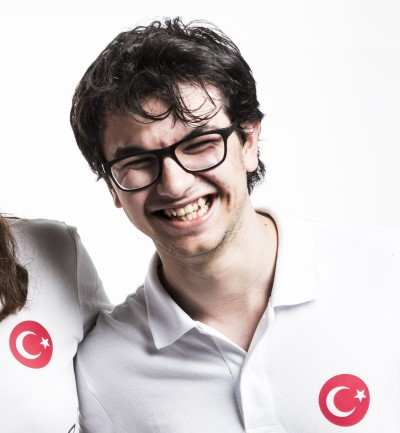
\includegraphics[width=.99\textwidth]{ahmet.jpg}
\end{subfigure}
\begin{subfigure}{.25\textwidth}
  \centering
  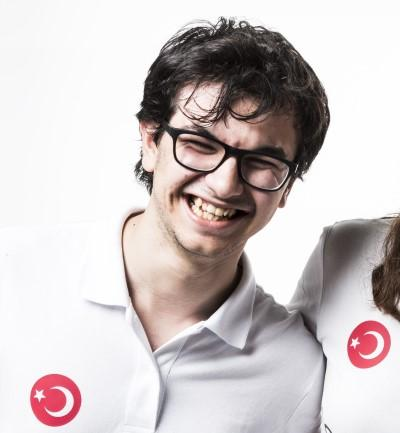
\includegraphics[width=.99\textwidth]{ahmet1.jpg}
\end{subfigure}
\begin{subfigure}{.25\textwidth}
  \centering
  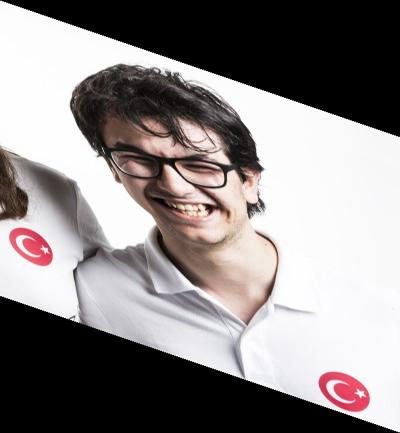
\includegraphics[width=.99\textwidth]{ahmet2.jpg}
\end{subfigure}
\begin{subfigure}{.25\textwidth}
  \centering
  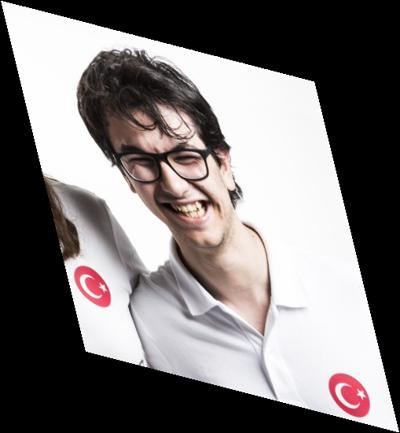
\includegraphics[width=.99\textwidth]{ahmet3.jpg}
\end{subfigure}%
\begin{subfigure}{.25\textwidth}
  \centering
  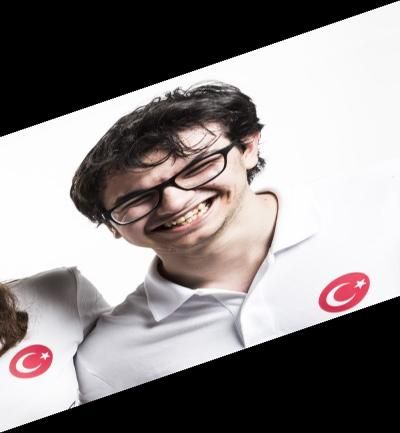
\includegraphics[width=.99\textwidth]{ahmet4.jpg}
\end{subfigure}
\begin{subfigure}{.25\textwidth}
  \centering
  
\includegraphics[width=.99\textwidth]{ahmet5.jpg}
\end{subfigure}
\begin{subfigure}{.25\textwidth}
  \centering
  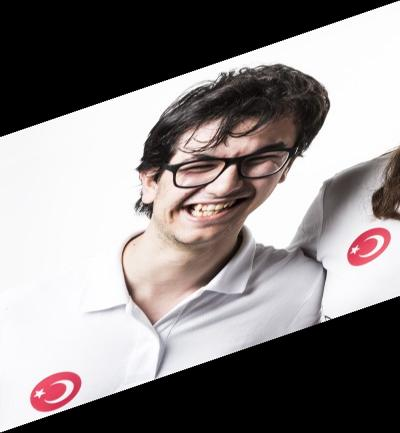
\includegraphics[width=.99\textwidth]{ahmet6.jpg}
\end{subfigure}%
\begin{subfigure}{.25\textwidth}
  \centering
  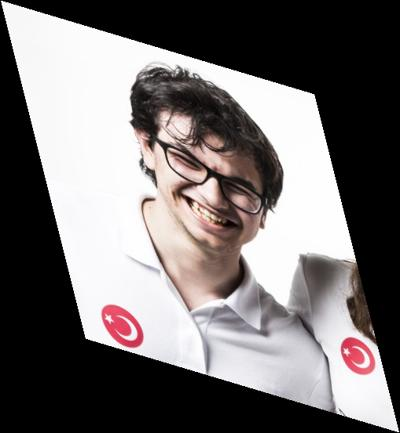
\includegraphics[width=.99\textwidth]{ahmet7.jpg}
\end{subfigure}
\begin{subfigure}{.25\textwidth}
  \centering
  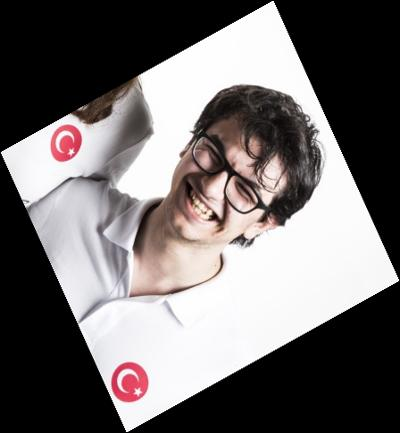
\includegraphics[width=.99\textwidth]{ahmet8.jpg}
\end{subfigure}
\caption{Sample original and warped images. First one is original and others are corresponding to matrices in the same order.}
\end{figure}

\newpage

\subsubsection{MATLAB Implementation}
\begin{lstlisting}[caption={MATLAB script for processing images taken from LFW database.},captionpos=b]
function [features_pos, features_neg] = get_training_features...
    (train_path_pos, train_path_neg,hog_template_size,hog_cell_size)
%This function returns the hog features of all positive examples and for
%negative examples
% INPUT:
%   . train_path_pos: a string which is path to the images of faces
%   . train_path_neg: a string which is path to images with no faces
%   . hog_template_size: size of hog template.
%   . hog_cell_size: the number of pixels in each HoG cell.
% OUTPUT
% . features_pos: a N1 by D matrix where N1 is the number of faces and D hog dimension
% . features_neg: a N2 by D matrix where N2 is the number of non-faces and D
image_files = dir( fullfile( train_path_pos, '*.jpg') );
num_images = length(image_files);
% create a matrix to store images
first_img = imread(strcat(image_files(1).folder, '\', image_files(1).name));
face_images = zeros([size(first_img), num_images], 'like', first_img); 
% store the images to use in warping
for i = 1:num_images
   face_images(:, :, i) = imread(strcat(image_files(i).folder, '\',...
       image_files(i).name)); 
end
% create affine2d objects used for warping
tform_reflection = affine2d([ -1 0 0; 0 1 0; 0 0 1]);
tform_shear = affine2d([1 .5 0; 0 1 0; 0 0 1]);
tform_shear2 = affine2d([1 .25 0; .25 1 0; 0 0 1]);
tform_shear3 = affine2d([1 -.5 0; 0 1 0; 0 0 1]);
tform_shear4 = affine2d([1 -.25 0; -.25 1 0; 0 0 1]);
tform_shear_reflect = affine2d([-1 .5 0; 0 1 0; 0 0 1]);
tform_shear_reflect2 = affine2d([-1 -.3 0; .25 1 0; 0 0 1]);
tform = affine2d([ 0.5*cos(pi/4) sin(pi/4)     0;
                  -sin(pi/4)     0.5*cos(pi/4) 0;
                   0             0             1]);
transforms = [tform_reflection, tform_shear, tform_shear2, tform_shear3,...
    tform_shear4, tform_shear_reflect, tform_shear_reflect2, tform];
% initialize features_pos with zeros
features_pos = zeros(num_images * (1 + length(transforms))...
    , (hog_template_size / hog_cell_size)^2 * 31);
% put the HoG for original face images 
for i = 1:num_images
    % calculate the HoG for face image
    hog = vl_hog(im2single(face_images(:, :, i)), hog_cell_size);
    % add the result to features_pos
    features_pos(i, :) = hog(:);
end
% iterate over all transforms and add HoG for warped faces
for i = 1:length(transforms)
    transform = transforms(i);
    warper = images.geotrans.Warper(transform, size(first_img));
    for j = 1:num_images
        % calculate the warped image
        warped_image = warp(warper, face_images(:, :, j));
        % resize the warped image to 36x36
        warped_image = imresize(warped_image, [36, 36]);
        % calculate the HoG for the warped face image
        hog = vl_hog(im2single(warped_image), hog_cell_size);
        % add the result to features_pos
        features_pos(i*num_images + j, :) = hog(:);
    end
end
\end{lstlisting}

\subsection{Negative Face Samples}
These samples are taken from provided non-face images. Images are randomly chosen from all non-face images and samples are taken from five different scales (0.25, 0.5, 1, 1.5 and 2). Random hog\_template\_size $\times$ hog\_template\_size parts of the scaled images are taken and used in the HoG calculation. Images are turned to gray-scale since all of our positive samples are in gray-scale. In each scaled versions of the randomly selected image $\lfloor \sqrt{w * h / hog\_template\_size^2}\rfloor$ windows are taken from the image where w and h represents dimensions of the image. I added this part to take samples depending on the size of the images since the differ in size.

\subsubsection{MATLAB Implementation}
\begin{lstlisting}[caption={Related part of the get\_training\_features function for getting HoG values of non-face images.},captionpos=b]
image_files = dir( fullfile( train_path_neg, '*.jpg' ));
num_images = length(image_files);
num_samples = 65000;
% counter for stopping at num_samples
sample_count = 0;
% different scales used for extracting, can be changed
scales = [.25, .5, 1, 1.5, 2];
% initialize  negative features matrix with zeros
features_neg = zeros(num_samples, (hog_template_size / hog_cell_size)^2 * 31);
% get num_samples samples    
while sample_count < num_samples
    % randomly select and image to sample windows from given dataset
    rand_img_index = random('unid', num_images);
    rand_img = imread(strcat(image_files(rand_img_index).folder,...
        '\', image_files(rand_img_index).name));
    % convert selected image to grayscale if it's rgb
    if size(rand_img, 3) == 3
        rand_img = rgb2gray(rand_img);
    end
    % take windows for different scales of randomly selected image
    for scale = scales
        % scale the image
        rand_scaled_img = imresize(rand_img, scale);
        % take the dimensions of the image
        [w, h] = size(rand_scaled_img);    
        % if dimensions are smaller than cell size we can't get any sample 
        if w < hog_template_size || h < hog_template_size
            continue
        end
        % determine how many samples will be taken
        num_sample_from_img = floor(sqrt(w * h / hog_template_size^2));
	% take num_sample_from_img  samples from the scaled image
        for i = 1:num_sample_from_img
            % randomly select window location 
            window_x = random('unid', w + 1 - hog_template_size);
            window_y = random('unid', h + 1 - hog_template_size);
            % increase the sample count
            sample_count = sample_count + 1;
            % calculate HoG for selected window
            hog = vl_hog(im2single(rand_scaled_img(...
                window_x:window_x+hog_template_size-1,...
                window_y:window_y+hog_template_size-1)), hog_cell_size);
            % add result to features_neg
            features_neg(i, :) = hog(:);
            % Stop if we react the wanted amount
            if sample_count >= num_samples
                break
            end
        end
        % Stop if we react the wanted amount
        if sample_count >= num_samples
            break
        end
    end
end
\end{lstlisting}
\section{Training Support Vector Machine using Features}
VL Feat toolbox is also used here to train a support vector machine, using positive and negative HoG features.

\subsection{MATLAB Implementation}

\begin{lstlisting}[caption={My implementation of svm\_training function.},captionpos=b]
function svmClassifier = svm_training(features_pos, features_neg)
% INPUT:
% . features_pos: a N1 by D matrix where N1 is the number of faces and D
%   is the hog feature dimensionality
% . features_neg: a N2 by D matrix where N2 is the number of non-faces and D
%   is the hog feature dimensionality
% OUTPUT:
% svmClassifier: A struct with two fields, 'weights' and 'bias' that are
%       the parameters of a linear classifier

% combine the features in one matrix to give to vl_svmtrain
X = [ features_pos ; features_neg ];
% create the label vector for indicating positive or negative feature 
Y = [ones(1, length(features_pos)) ,  -ones(1, length(features_neg))];
lambda = 0.00001;
% Function wants an D by N matrix (D: feature dimensions, N: feature count)
% so input the transpose of X
[w, b] = vl_svmtrain(X', Y, lambda);
svmClassifier = struct('weights',w,'bias',b);
end
\end{lstlisting}

\newpage

\subsection{Visualizatioın of SVM Classifier by its Weights}

\begin{figure}[!htb]
\begin{subfigure}{.40\textwidth}
  \centering
  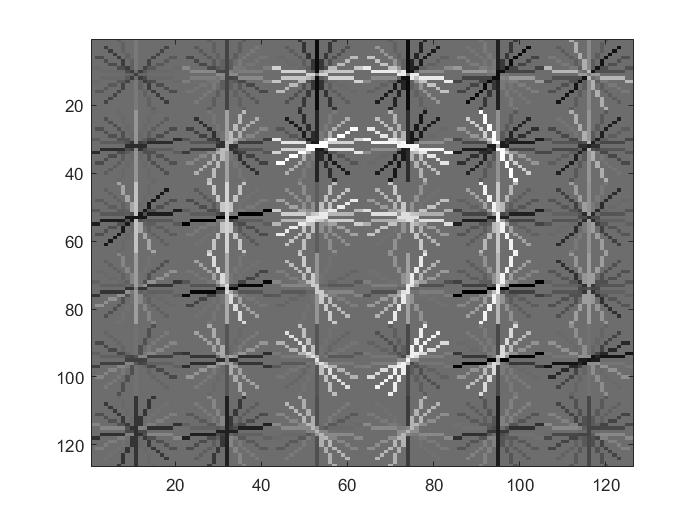
\includegraphics[width=.99\textwidth]{hogs_6_lfw.jpg}
\caption{LFW dataset with cell size 6.}
\end{subfigure}
\begin{subfigure}{.40\textwidth}
  \centering
  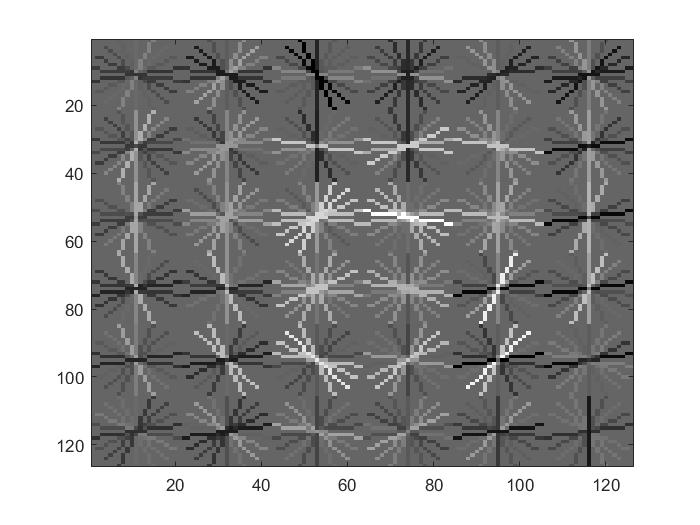
\includegraphics[width=.99\textwidth]{hogs_6.jpg}
\caption{Caltech dataset with cell size 6.}
\end{subfigure}
\begin{subfigure}{.44\textwidth}
  \centering
  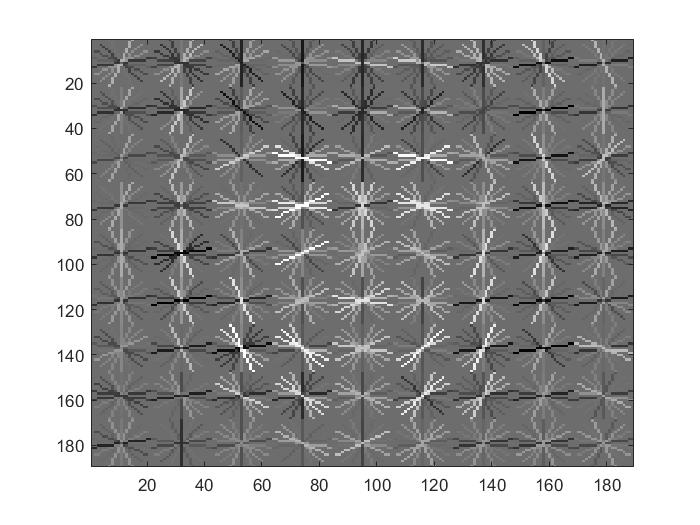
\includegraphics[width=.99\textwidth]{hogs_4.jpg}
\caption{Caltech dataset with cell size 4.}
\end{subfigure}
\begin{subfigure}{.54\textwidth}
  \centering
  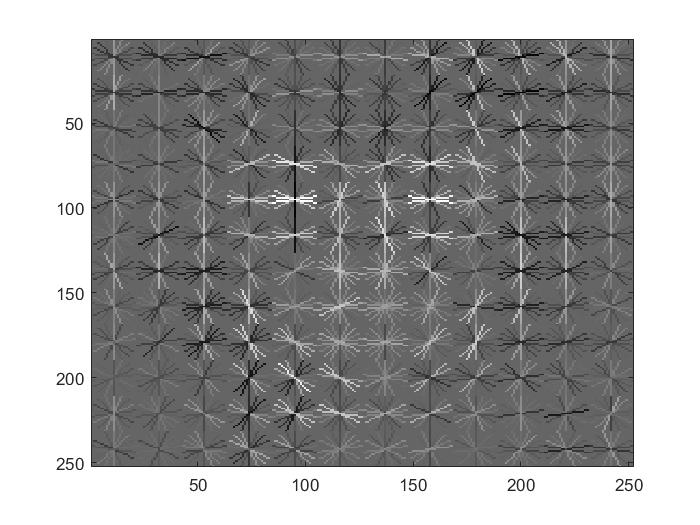
\includegraphics[width=.99\textwidth]{hogs_3.jpg}
\caption{Caltech dataset with cell size 3.}
\end{subfigure}
\caption{Visualizations of SVM classifiers using its weights with different HoG cell sizes.}
\end{figure}

Higher weights are represented with higher brightness in the figures. Since all of our positive training data was upfront face images, weights are bigger on the middle part of the image since faces were in the middle of the image in most of the cases. Also, you can see the increased concentration on distinctive parts like eyes and face borders. The difference between LFW dataset and Caltech dataset is also important. In Caltech dataset, faces are more uniform, their angle and the location of the face is almost identical across all images. However, LFW dataset has more varying head images and heads cover a smaller area in images. So, the concentrated part is smoother compared to Caltech dataset.


\section{Testing SVM Classifier on Training Data}
Trained classifier is tested on training data and the results will be evaluated from four aspects based on the number of true positives, false positives, true negatives and false negatives:

\begin{enumerate} 
\item Accuracy: Overall, how often is the classifier correct?  (TP+TN)/(TP+TN+FP+FN)
\item Recall: When it's actually a face, how often does it predict face?  TP/(TP+FN)
\item True Negative Rate: When it's actually non-face, how often does it predict non-face? TN/(TN+FP)
\item Precision: When it predicts face, how often is it correct? TP/(TP+FP)
\end{enumerate}

SVM classifier has the results, accuracy = 0.9999, recall = 0.99997, tn\_rate = 0.99985 and precision = 0.99983 calculated using the counts of TP, TN, FP and FN.

\subsection{MATLAB Implementation}
\begin{lstlisting}[caption={My implementation of classifier\_performance function.},captionpos=b]
function [accuracy,recall,tn_rate,precision] = classifier_performance(svmClassifier,features_pos,features_neg)
% initialize counters
true_positive = 0;
false_negative = 0;
false_positive = 0;
true_negative = 0;
% extract weights and bias
w = svmClassifier.weights;
b = svmClassifier.bias;
% check for positive images
for i = 1:length(features_pos)
   if features_pos(i, :) * w + b >= 0
       % face is recognized as face: increase true positive
       true_positive = true_positive + 1;
   else
       % face is not recognized: increase false negative
       false_negative = false_negative +1;
   end
end
% check for negative images
for i = 1:length(features_neg)
   if features_neg(i, :) * w + b >= 0
       % non-face recognized as face: increase false positive
       false_positive = false_positive + 1;
   else
       % non-face is not recognized: increase true negative
       true_negative = true_negative +1;
   end
end
% calculate values from counters
accuracy = (true_positive + true_negative) /...
    (true_positive + true_negative + false_positive + false_negative);
recall = true_positive / (true_positive + false_negative);
tn_rate = true_negative / (true_negative + false_positive);
precision = true_positive / (true_positive + false_positive);
end
\end{lstlisting}


\section{Analyze Classifier Performance on the Test Data using Sliding Windows}


\subsection{MATLAB Implementation}

\begin{lstlisting}[caption={My implementation of run\_detector function.},captionpos=b]
function [bboxes, confidences, image_ids] = ....
    run_detector(test_data_path, svmClassifier, hog_template_size,hog_cell_size)
% get all jpg files on data path
test_scenes = dir( fullfile( test_data_path, '*.jpg' ));
num_images = length(test_scenes);
%initialize these as empty and incrementally expand them.
bboxes = zeros(0,4);
confidences = zeros(0,1);
image_ids = cell(0,1);
% iterate over all images
for i = 1:num_images
    % read the image file
    image_name = test_scenes(i).name;
    fprintf('Detecting faces in %s\n', image_name);
    img = imread( fullfile( test_data_path, test_scenes(i).name ));
    %  get the confidences and bounding boxes for this image
    [cur_confidences,cur_bboxes] =...
       Detector(img, svmClassifier, hog_template_size,hog_cell_size);
    cur_image_ids = cell(0,1);
    cur_image_ids(1:size(cur_bboxes,1)) = {test_scenes(i).name}; 
    % add results to matrices
    bboxes      = [bboxes;      cur_bboxes];
    confidences = [confidences; cur_confidences];
    image_ids   = [image_ids;   cur_image_ids];
end
end
\end{lstlisting}

\begin{lstlisting}[caption={My implementation of Detector function.},captionpos=b]
function [cur_confidences,cur_bboxes] = ...
    Detector(img, svmClassifier, hog_template_size,hog_cell_size)
% initialize bounding boxes and confidences matrices
% bboxes will store x_min, y_min, x_max, y_max  hence has 4 columns
cur_bboxes = zeros(0,4);
cur_confidences = zeros(0,1);
% convert image to grayscale if it's rgb
if size(img, 3) == 3
    img = rgb2gray(img);
end
% calculate the size of patch based on template and cell sizes
size_patch = hog_template_size / hog_cell_size;
% extract weights and bias
w = svmClassifier.weights;
b = svmClassifier.bias;
scale = 1.0;
% iterate over all scales
for i = 1:20
    % scale the image
    scaled_img = imresize(img, scale);
    % calculate the hog for whole scaled image
    hog = vl_hog(im2single(scaled_img), hog_cell_size);
    % get dimensions of hog matrix
    [size_y, size_x, ~] = size(hog);
    % iterate over all patches
    % equivalent to iterating over the image with cell_size
    for x = 1:(size_x - size_patch + 1)
        for y = 1:(size_y - size_patch + 1)
            % get hog of the patch from hog of the image
            hog_of_patch = hog(y:y+size_patch-1, x:x+size_patch-1, :);
            % vectorize the hog for multiplication
            hog_row_vector = hog_of_patch(:)';
            % check for face detection      
            confidence = hog_row_vector * w + b;
            % add detection to matrices if it has confidence more than a threshold
            if confidence >= 1.4
                cur_bboxes = [1 + (x-1)*hog_cell_size/scale,...
                    1+(y-1)*hog_cell_size/scale,...
                    (hog_template_size+(x-1)*hog_cell_size)/scale,...
                    (hog_template_size+(y-1)*hog_cell_size)/scale...
                    ; cur_bboxes];
                cur_confidences = [ confidence ; cur_confidences];
            end
        end
    end
    scale = scale * 0.9;
end 
% Apply non-max supression to detected faces
[cur_bboxes, cur_confidences] = ...
    nonMaximum_Suppression(cur_bboxes, cur_confidences,size(img));
end
\end{lstlisting}

\subsection{Sample Results}
These are sample results for SVM classifier trained with Caltech face dataset with no image warping, using 65,000 negative samples and cell size 6. Classifier is run on multi-scale. 1.9 confidence threshold is used.

\begin{figure}[!htb]
 \centering
  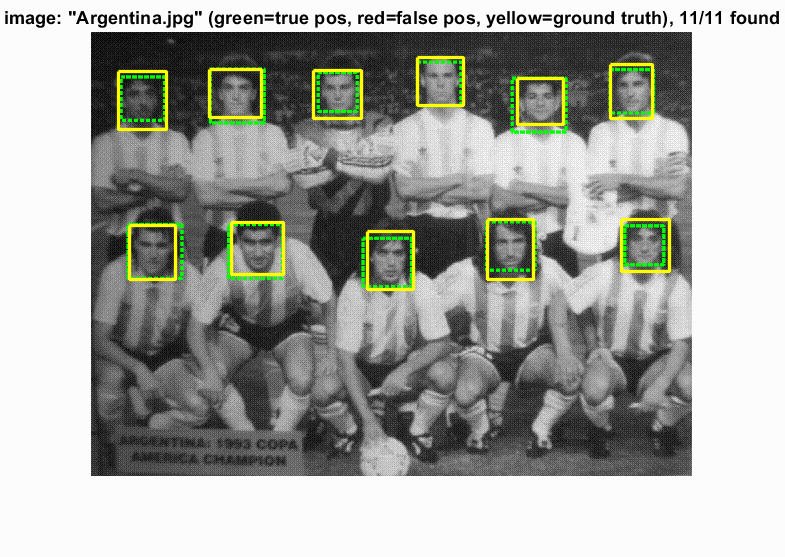
\includegraphics[width=.8\textwidth]{sample1.png}
\end{figure}%
\begin{figure}[!htb]
 \centering
  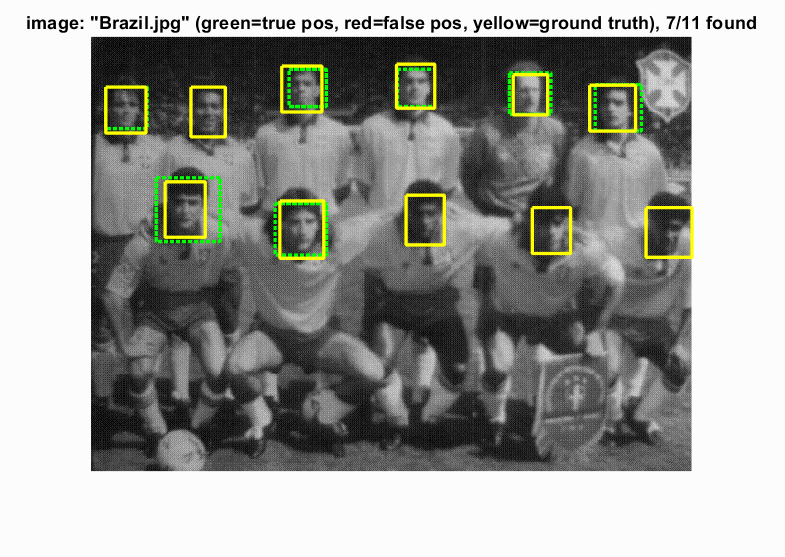
\includegraphics[width=.9\textwidth]{sample2.png}
\end{figure}%
\begin{figure}[!htb]
 \centering
  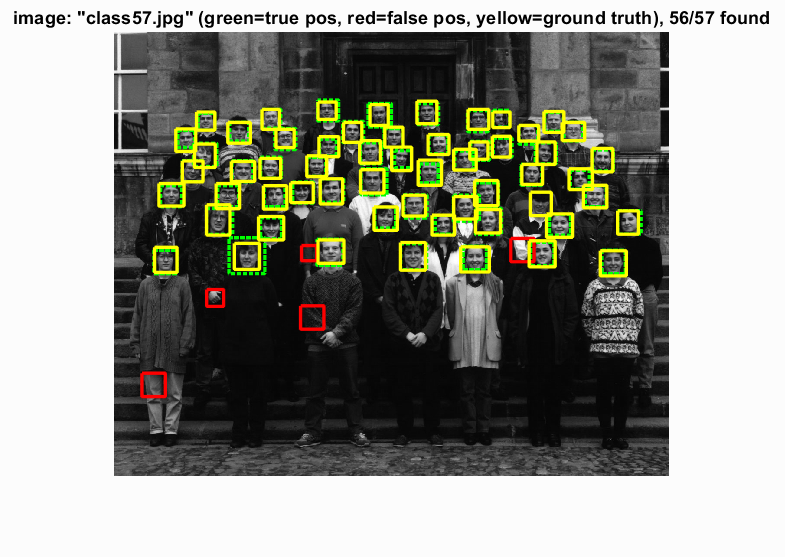
\includegraphics[width=.9\textwidth]{sample3.png}
\end{figure}%
\newpage
\begin{figure}[!htb]
 \centering
  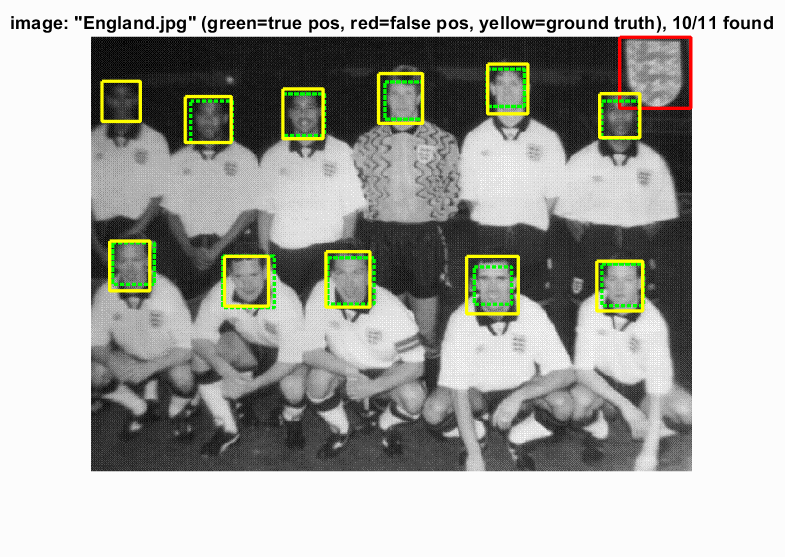
\includegraphics[width=.92\textwidth]{sample4.png}
\end{figure}%
\begin{figure}[!htb]
 \centering
  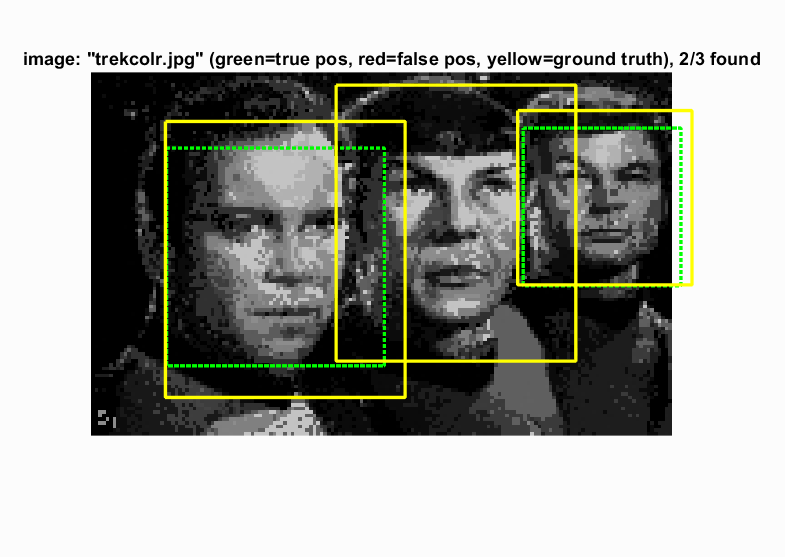
\includegraphics[width=.92\textwidth]{sample5.png}
\end{figure}%

\newpage

\section{Dimensionality Reduction using PCA}
I implemented PCA dimensionality reduction algorithm with threshold of 0.9. I only run it once and it took almost an hour. It resulted poorly compared to the default detection(without using PCA). Huge performance difference can be caused by some other factor but I couldn't find it since it tooks too much time.


\begin{figure}[!htb]
\begin{subfigure}{.48\textwidth}
  \centering
  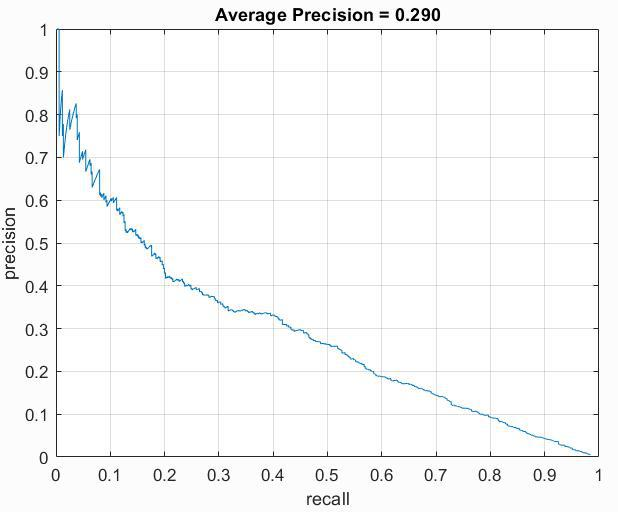
\includegraphics[width=.99\textwidth]{pca.jpg}
\end{subfigure}
\begin{subfigure}{.48\textwidth}
  \centering
  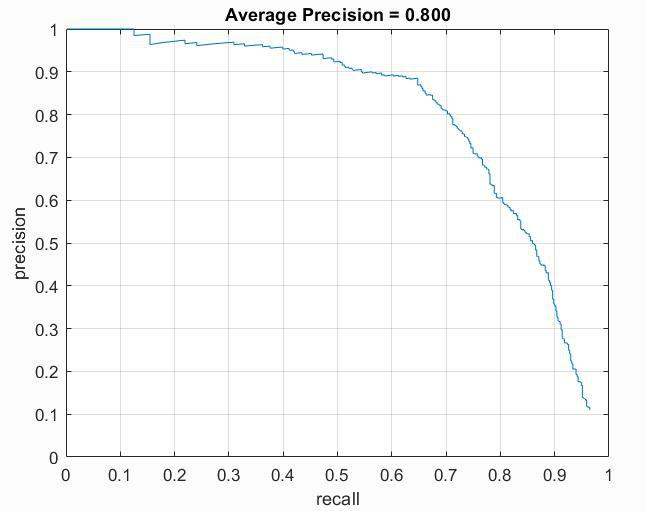
\includegraphics[width=.99\textwidth]{non_pca.jpg}
\end{subfigure}
\caption{Difference between precision recall graph. Left one is with PCA Dimensionality reduction.}
\end{figure}

\subsection{MATLAB Implementation}
\begin{lstlisting}[caption={My implementation of Detector function.},captionpos=b]
function pca_coeff = pca_components(features)
threshold = 0.9;
% substract mean from features 
features = features - mean(features);
% calculate covariance matrix
covariance_mat = features'*features./length(features);
% find eigen values and corresponding eigen vectors
[eig_vectors, eig_values_matrix] = eig(covariance_mat);
% sort eigen values in descending order, save original index of the value 
eig_values = diag(eig_values_matrix);
[eig_values,sorted_indices] = sort(eig_values, 'descend');
% calculate cumulative sum to check for threshold condition
cumsums = cumsum(eig_values);
% calculate how many eigen vectors to take
index = 1;
while cumsums(index) < threshold * cumsums(end)
    disp(cumsums(index))
    index = index + 1;
end
% initialize pca_coefficient matrix with zeros
pca_coeff = zeros(length(eig_values), index);
% copy eigenvectors to pca_coefficients
for i = 1:index
    pca_coeff(: ,i) = eig_vectors(:, sorted_indices(i));
end
end
\end{lstlisting}

\section{Discussion About Classifier Performance}
Given results are obtained using the Caltech dataset for positive images without image warping, 65,000 negative samples for positive images. HoG cell size 6 is used, detections are thresholded with confidence 1.4 and faces are detected in multiscale. Tests are run on given MIT+CMU test scenes with the assignment. These specifications are true unless otherwise specified. The values given in the text are the average of 5 runs, given graphs are the graphs of the closest run to the average.

\begin{figure}[!htb]
 \centering
  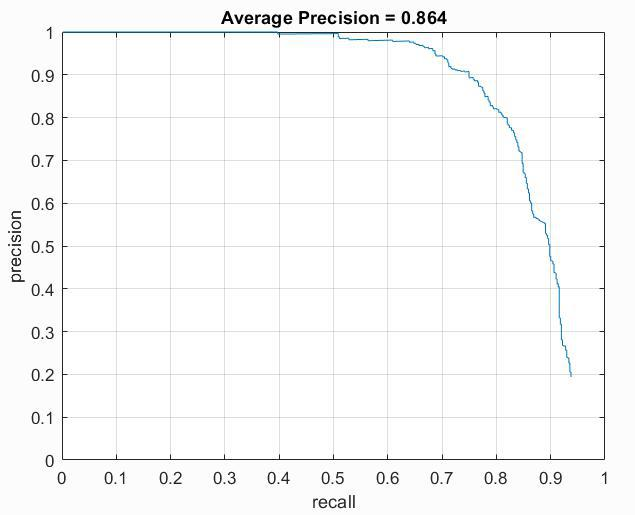
\includegraphics[width=.92\textwidth]{final.jpg}
\caption{Precision-recall graph for my final SVM Classifier on MIT-CMU test scenes.}
\end{figure}%

As it can seen from the graph, precision value decreases when recall increases. Since recall is checking for the ratio of true positives and sum of true positives and false negatives, getting false positive does not affect this metric. Face parts are getting decent confidence values from our SVM classifier, bigger problem is the classifier produce false positives as we decrease the confidence threshold. So, getting a good recall means getting lots of false positives, hence, low precision. 

\subsection{Effects of Multi-scale Detection}

As you can see from graphs, multi-scale detection increases precision of our SVM classifier drastically. Since we used 36x36 face images to train the classier it will only detect faces closer to that size. To solve this problem we will use the same windows size, however, we will use this sliding windows on different scaled versions of the images. This will enable us to detect bigger and smaller (I didn't use scales bigger than 1 since 36x36 is already too small bu can be done) faces.

\begin{figure}[!htb]
\begin{subfigure}{.48\textwidth}
  \centering
  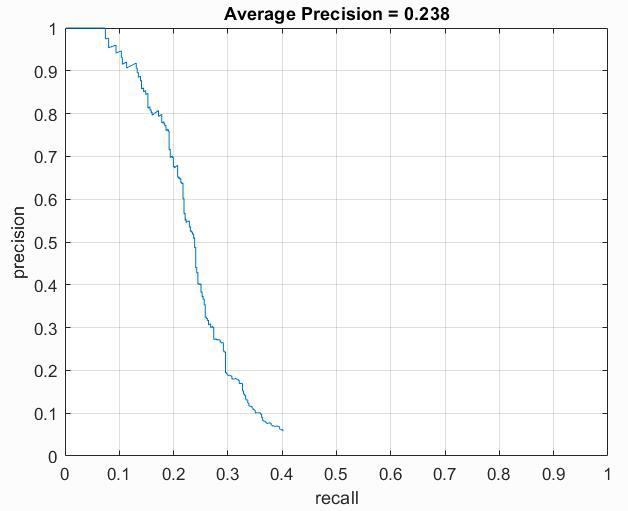
\includegraphics[width=.99\textwidth]{no_scale.jpg}
\end{subfigure}
\begin{subfigure}{.48\textwidth}
  \centering
  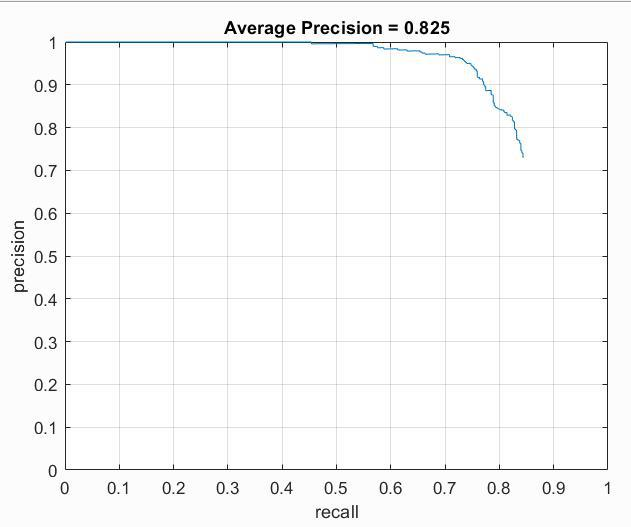
\includegraphics[width=.99\textwidth]{step3.jpg}
\end{subfigure}
\caption{Difference between precision recall graph. Left one is with detection in one scale, right is multi-scale.}
\end{figure}

\subsection{Effects of Adding More Faces Using Image Warping}

Adding more positive samples with image warping decreased SVM's precision on MIT-CMU test scenes. On average, SVM trained with both original and warped face images discussed above, it has a confidence of 0.770. This decrease might be caused from using wrong transformations, or faces obtained with these transformations might be rare in the test scenes. 

\begin{figure}[!htb]
\begin{subfigure}{.48\textwidth}
  \centering
  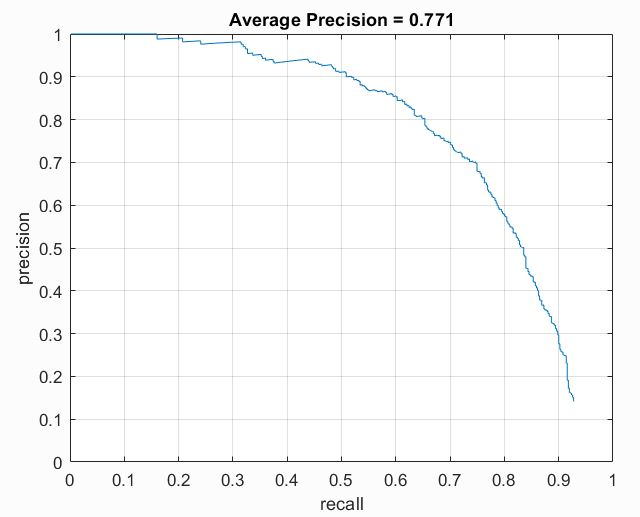
\includegraphics[width=.99\textwidth]{warped.jpg}
\end{subfigure}
\begin{subfigure}{.48\textwidth}
  \centering
  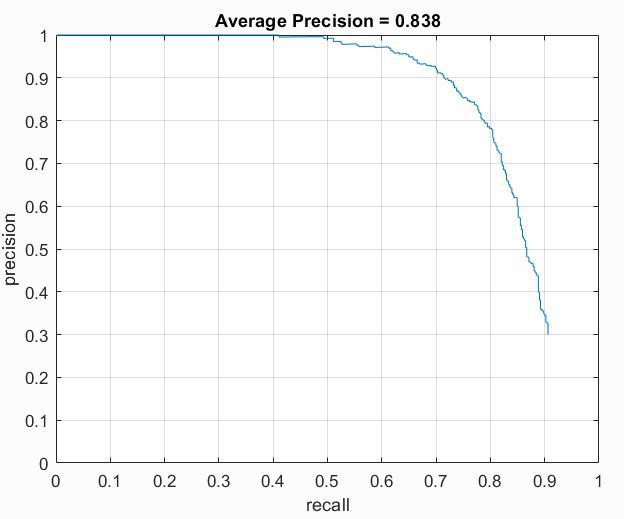
\includegraphics[width=.99\textwidth]{nowarp.jpg}
\end{subfigure}
\caption{Difference between precision recall graph. Left one is trained with warped images.}
\end{figure}

\newpage

\subsection{Effect of HoG Cell Size Selection}

The average results for different HoG cell sizes (5 runs) are as follows:
\begin{enumerate} 
\item 6: 0.83224
\item 3: 0.8256
\item 4: 0.7608
\item 9: 0.706
\item 12: 0.702
\end{enumerate}

As you can see there is a pattern, as cell size decreases precision increases. However, this pattern does not hold for cell size 6. This might be caused from randomness in the training since we get negative sample randomly.

\subsection{Performance Difference Between Two Face Datasets}

SVMs trained with Caltech dataset is more successful than SVMs trained with LFW dataset. Caltech images are more uniform and has the faces with exactly the same orientation and location. Even though LFW dataset is constructed using Deep Funnelling, faces cover smaller size of the images and there are many different orientations for the images. So, this might be the reason why Caltech dataset is more appropriate for face recognition using SVM and sliding window.

\begin{figure}[!htb]
\begin{subfigure}{.48\textwidth}
  \centering
  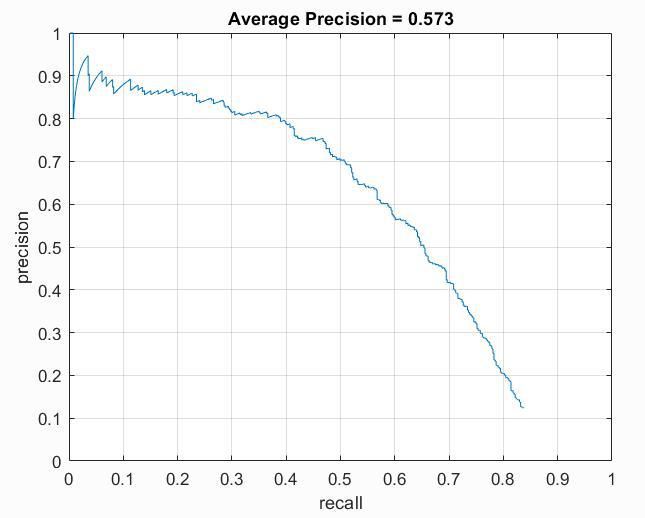
\includegraphics[width=.99\textwidth]{lfw.jpg}
\end{subfigure}
\begin{subfigure}{.48\textwidth}
  \centering
  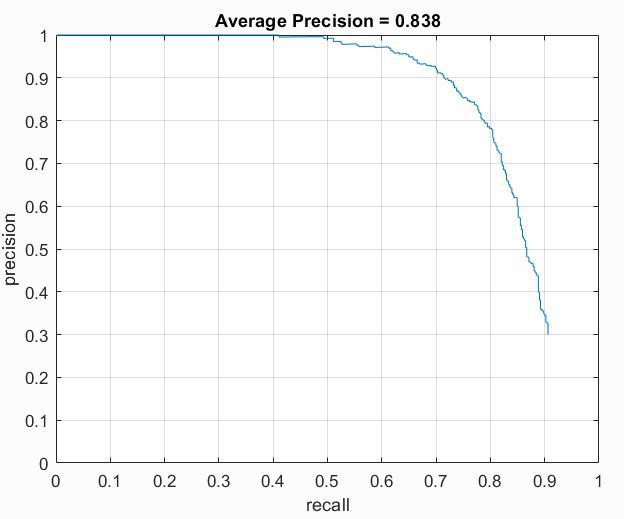
\includegraphics[width=.99\textwidth]{nowarp.jpg}
\end{subfigure}
\caption{Difference between precision recall graph. Left one is trained with LFW dataset.}
\end{figure}

\subsection{Effects of Using Smaller Step Size}
I also implemented the run\_detector method with 1 step size by calculating the multiple times. However, it didn't have a great impact on the performance but it made the algorithm run significantly slower, so, I didn't use it. It only has a small impact of 0.001-0.002 on the confidence. I couldn't see its difference visually on results.

\newpage

\section{Results for Extra Test Cases}
For these images 1.9 confidence threshold is used.

\begin{figure}[!htb]
 \centering
  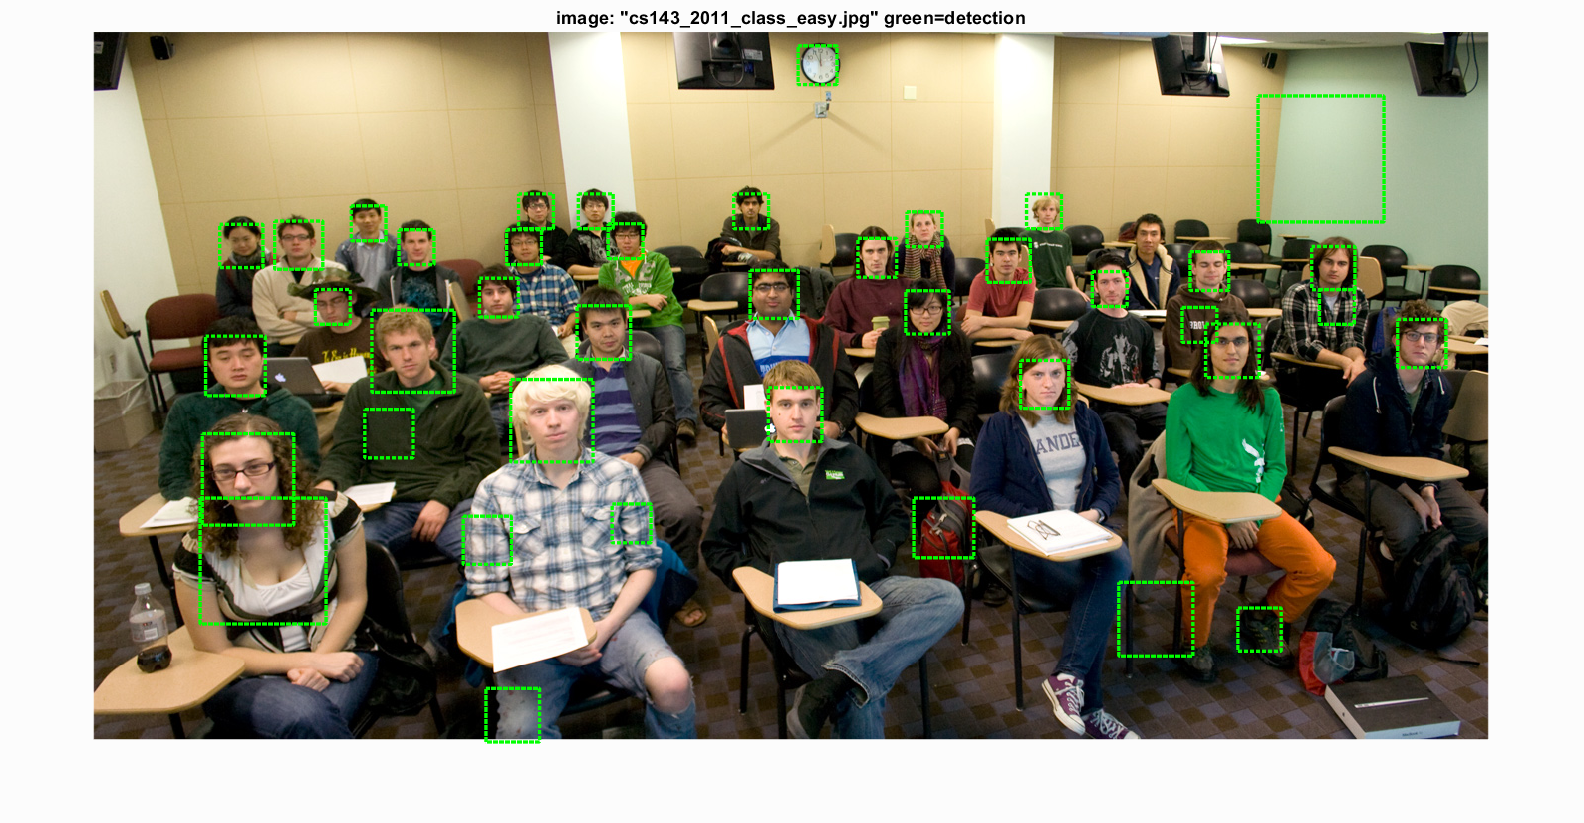
\includegraphics[width=.99\textwidth]{extra_easy1.png}
\end{figure}%
\begin{figure}[!htb]
  \centering
  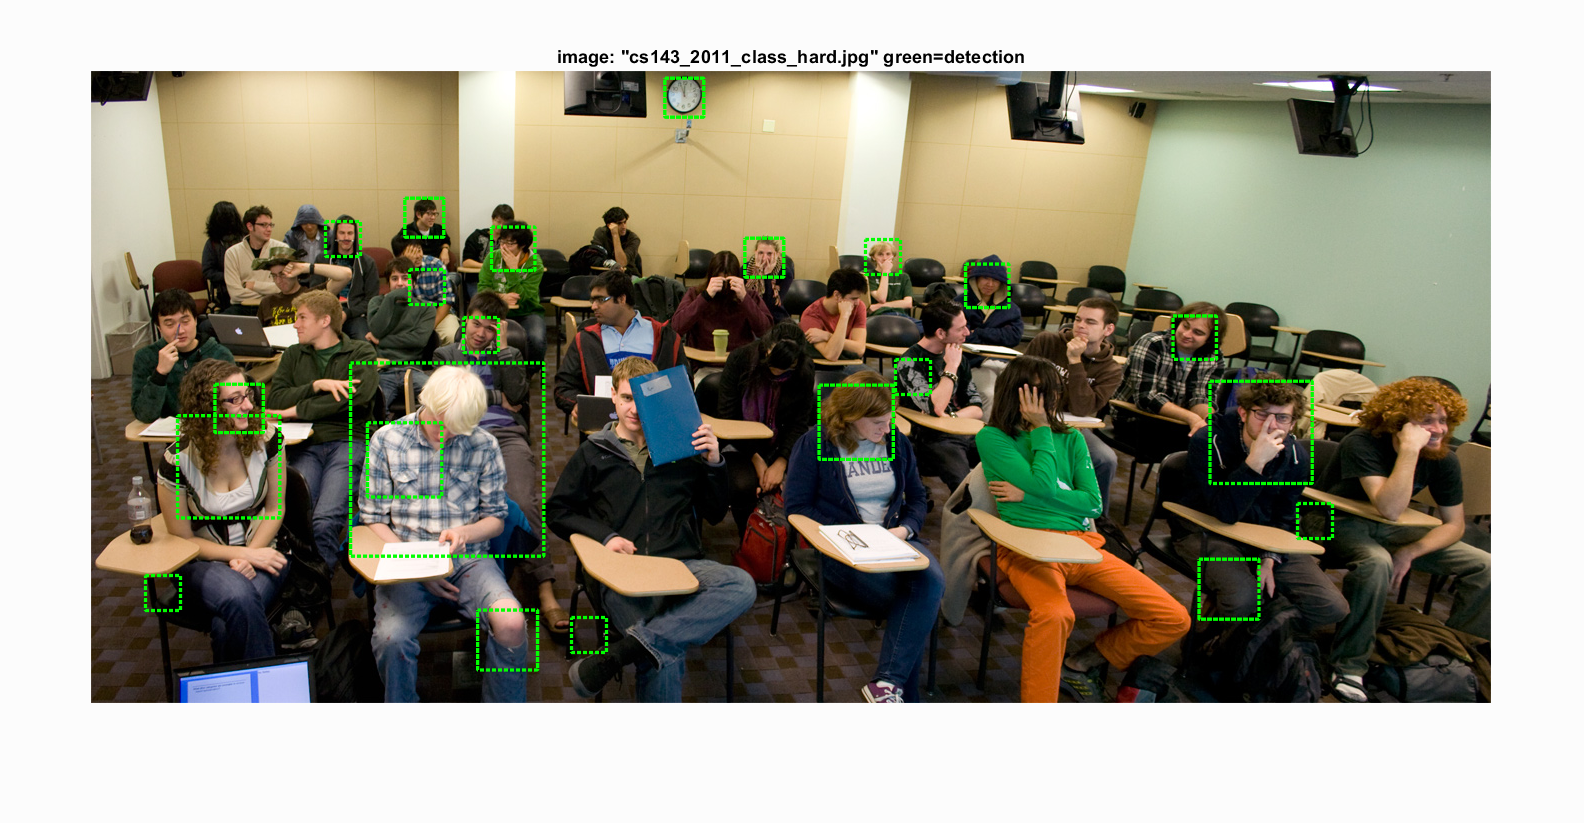
\includegraphics[width=.99\textwidth]{extra_hard1.png}
\end{figure}%
\newpage
\begin{figure}[!htb]
  \centering
  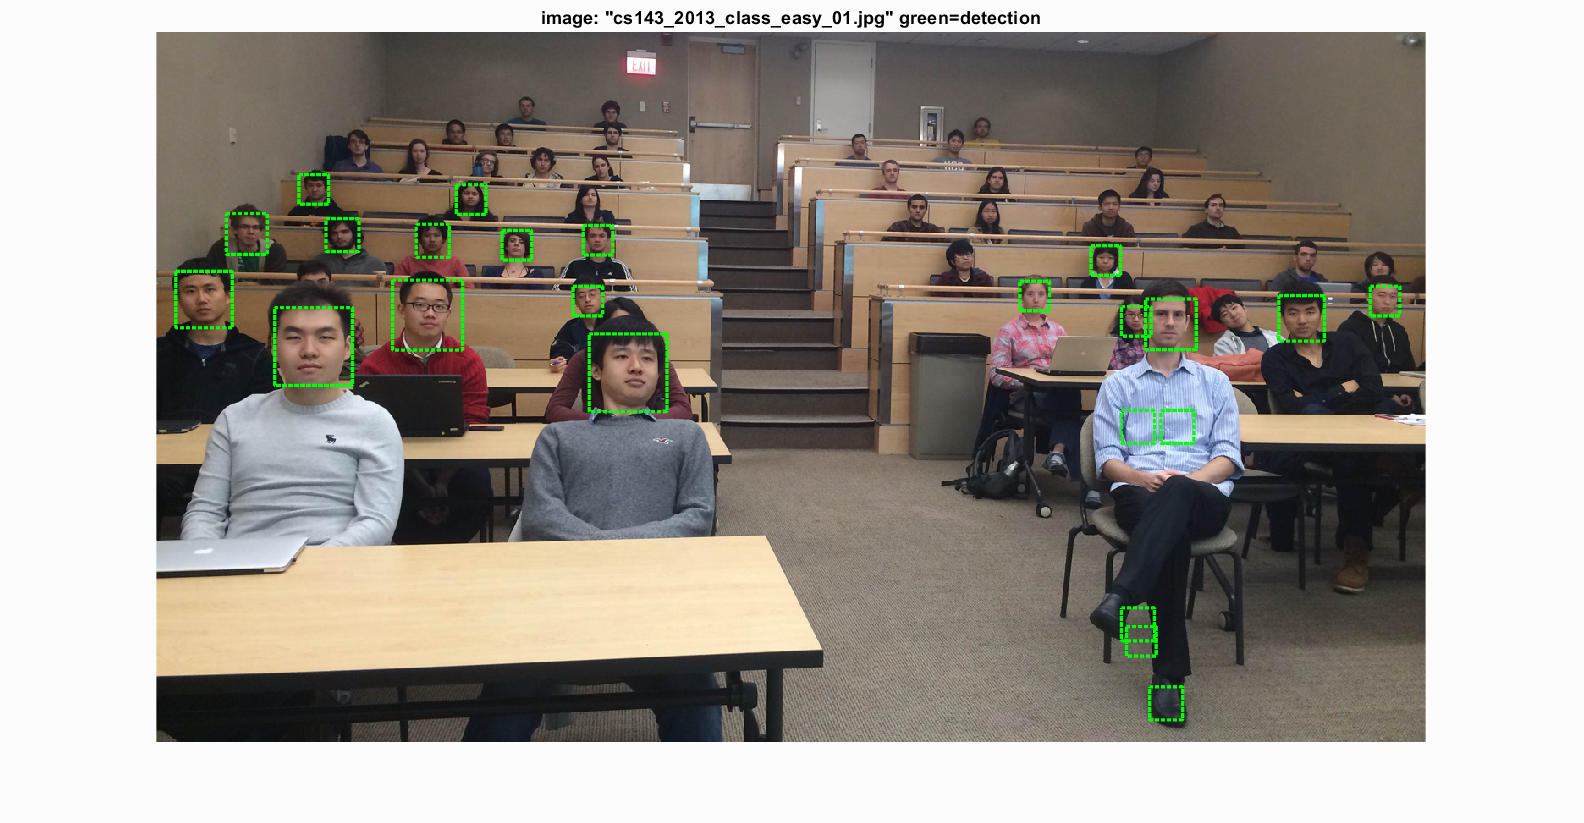
\includegraphics[width=.99\textwidth]{extra_easy2.png}
\end{figure}%

\begin{figure}[!htb]
  \centering
  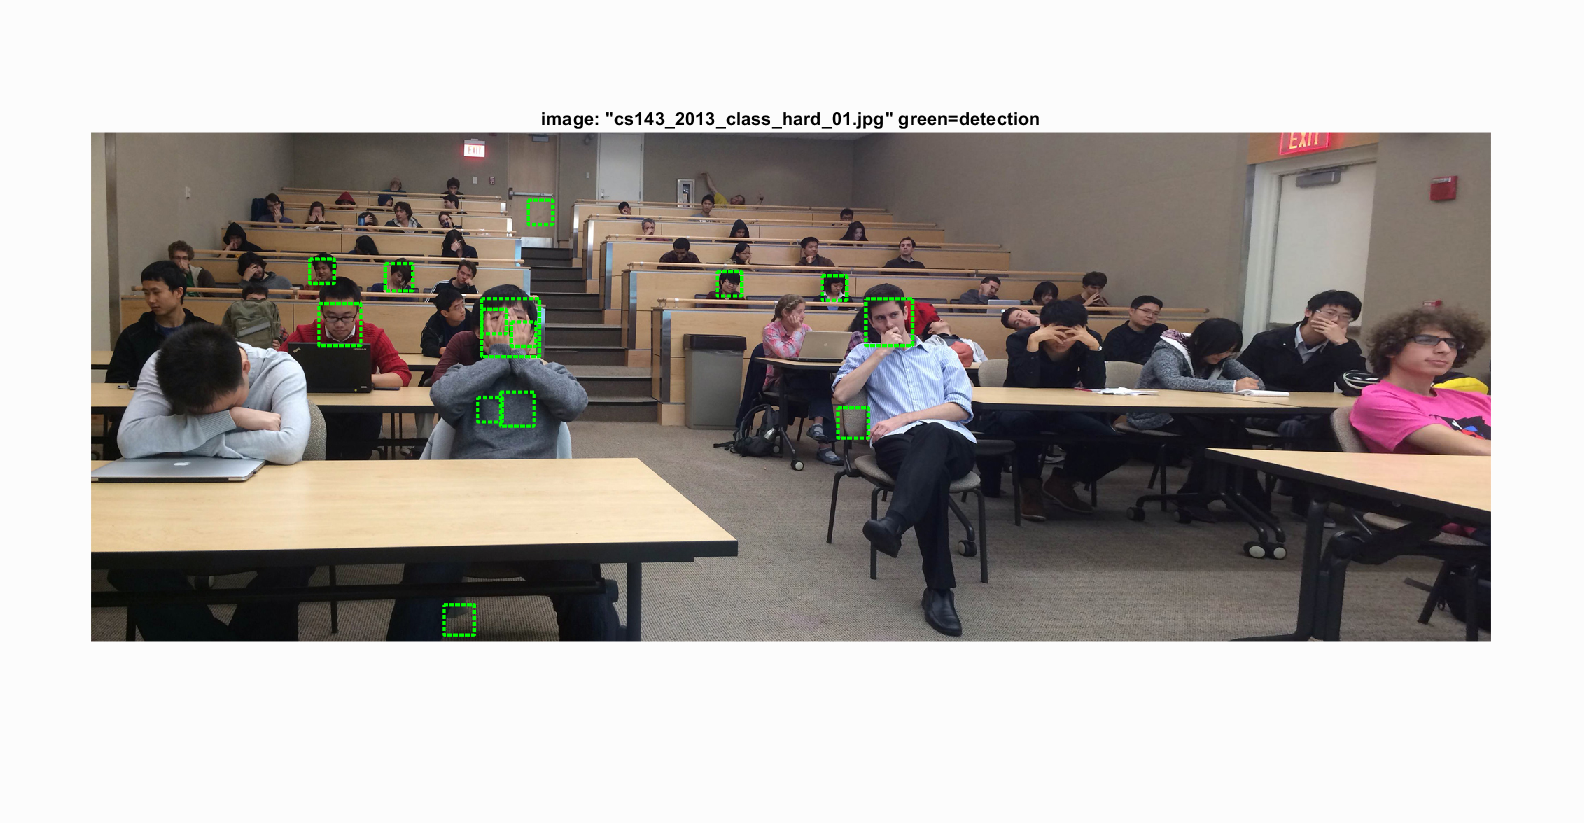
\includegraphics[width=.99\textwidth]{extra_hard2.png}
\end{figure}%

\begin{figure}[!htb]
 \centering
  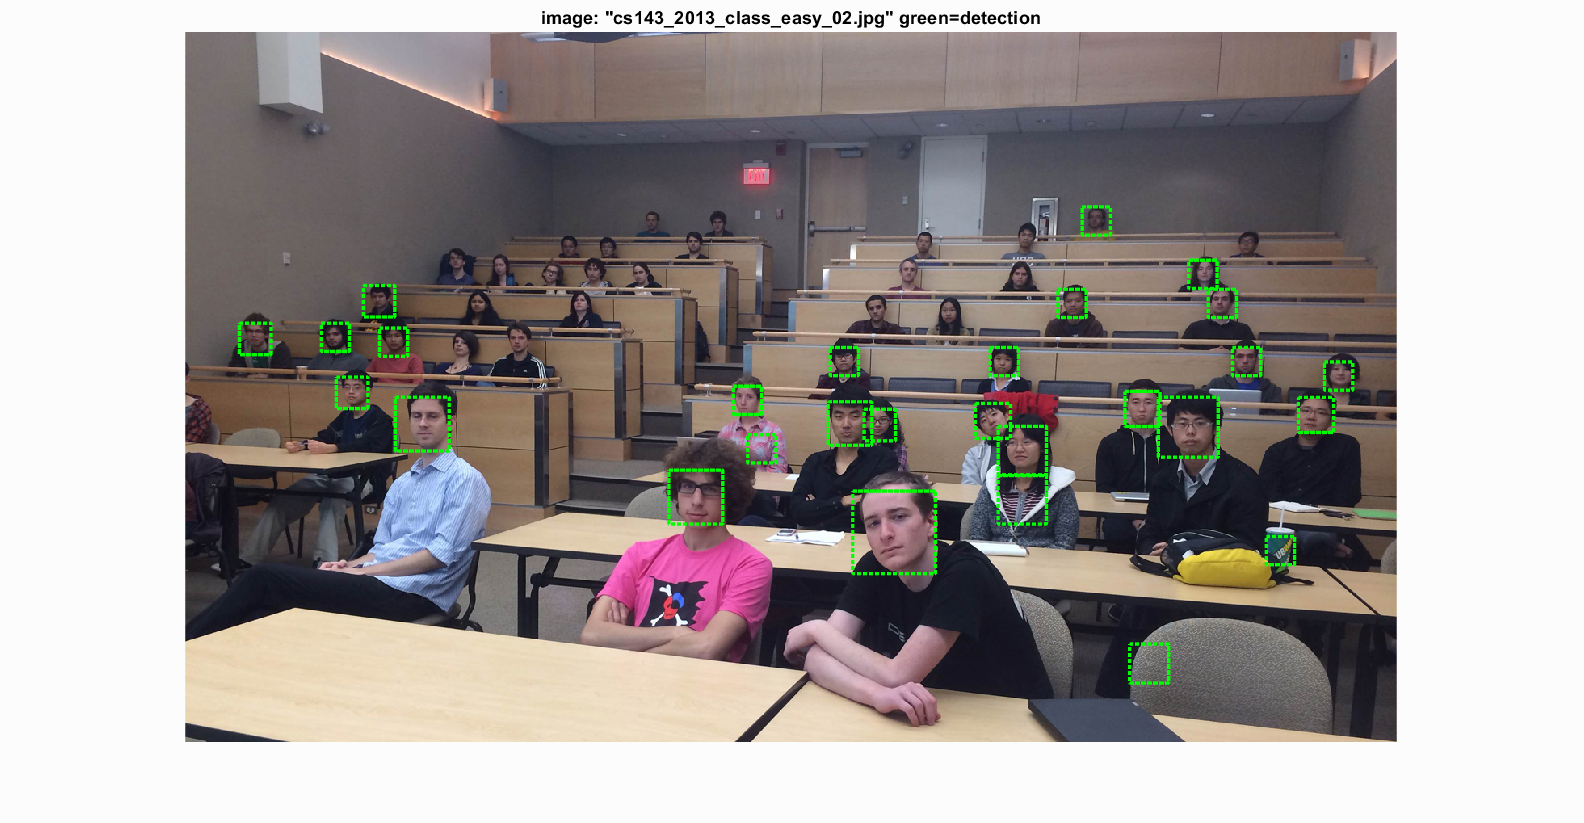
\includegraphics[width=.99\textwidth]{extra_easy3.png}
\end{figure}%
\begin{figure}[!htb]
  \centering
  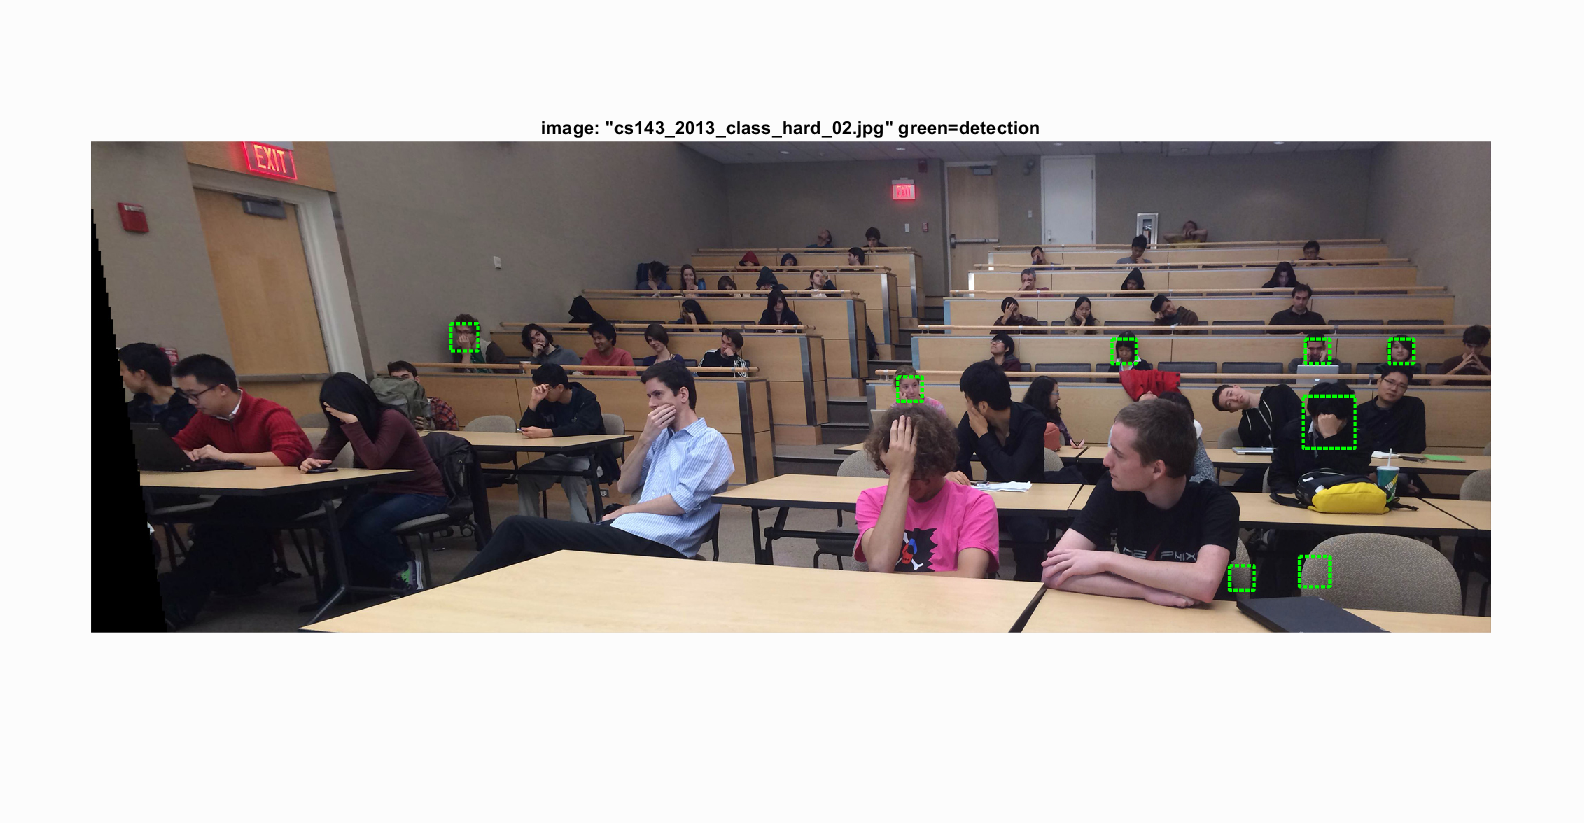
\includegraphics[width=.99\textwidth]{extra_hard3.png}
\end{figure}%
\newpage
\begin{figure}[!htb]
  \centering
  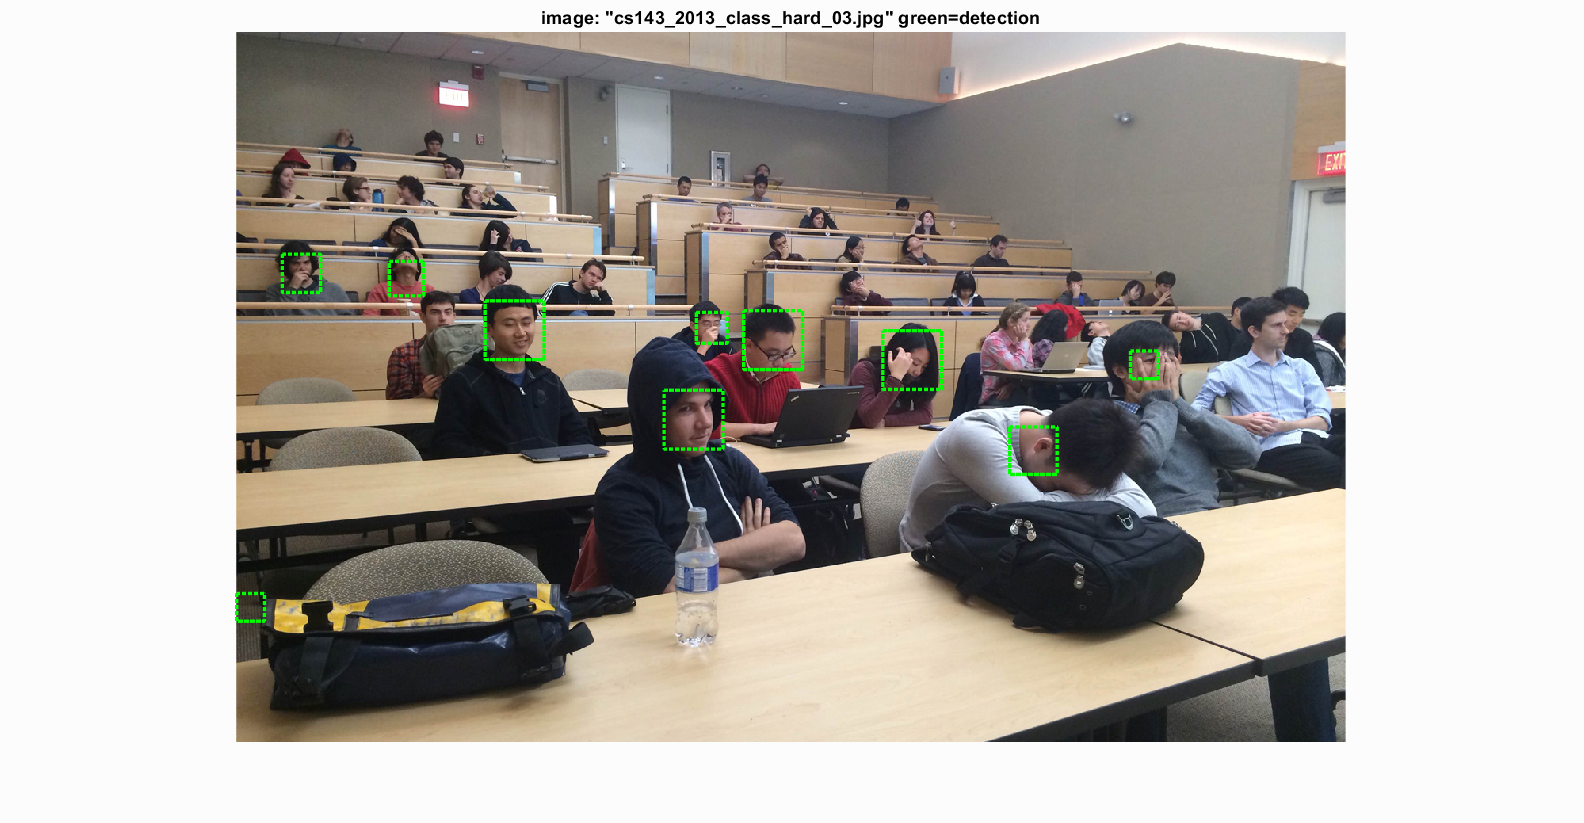
\includegraphics[width=.99\textwidth]{extra_hard4.png}
\end{figure}%

\begin{figure}[!htb]
  \centering
  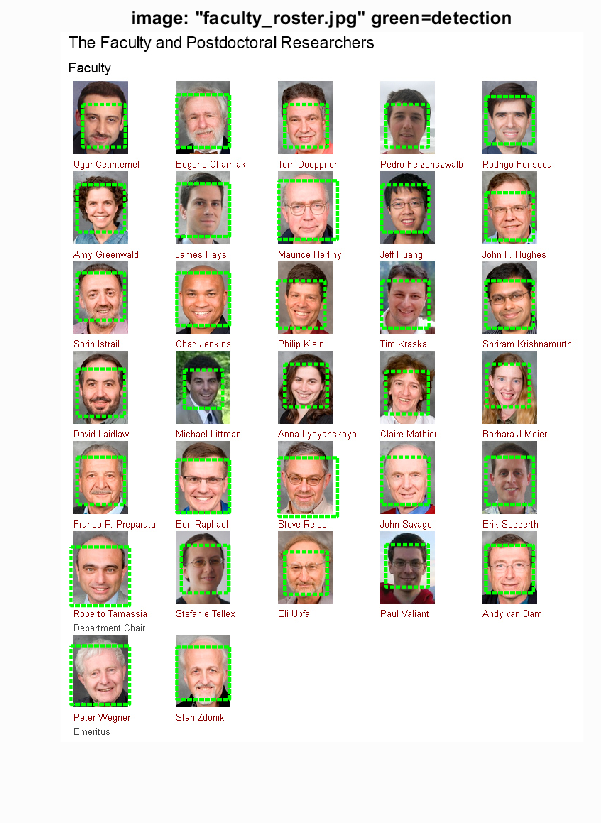
\includegraphics[width=.99\textwidth]{roster.png}
\end{figure}%



\end{document}